\section{Organization and Management (4 pages)}
\label{sec:fdsp-apa-org}


%%%%%%%%%%%%%%%%%%%%%%%%%%%%%%%%%%%%%
\subsection{APA Consortium Organization}
\label{sec:fdsp-apa-org-consortium}
The APA Consortium comprises 21 institutions, of which 13 from the US, 7 from the UK, and one from the Czech Republic. The Consortium is organized along the main deliverables, which are the final design of the APA and the APA production and assembly procedures. Since the two main centers for APA construction are expected to be located in the US and the UK, there are usually two leaders of each working group, representing the main stakeholders (Fig.~\ref{fig:APAorg}). This is particularly important to ensure that common procedures and tooling are developed. 

%\fixme{I asked Maxine about standardized org charts for each consortium. It would be nice to have these. Anne}

\begin{dunefigure}[APA Consortium Organizational Chart]{fig:APAorg}
{APA Consortium Organizational Chart}
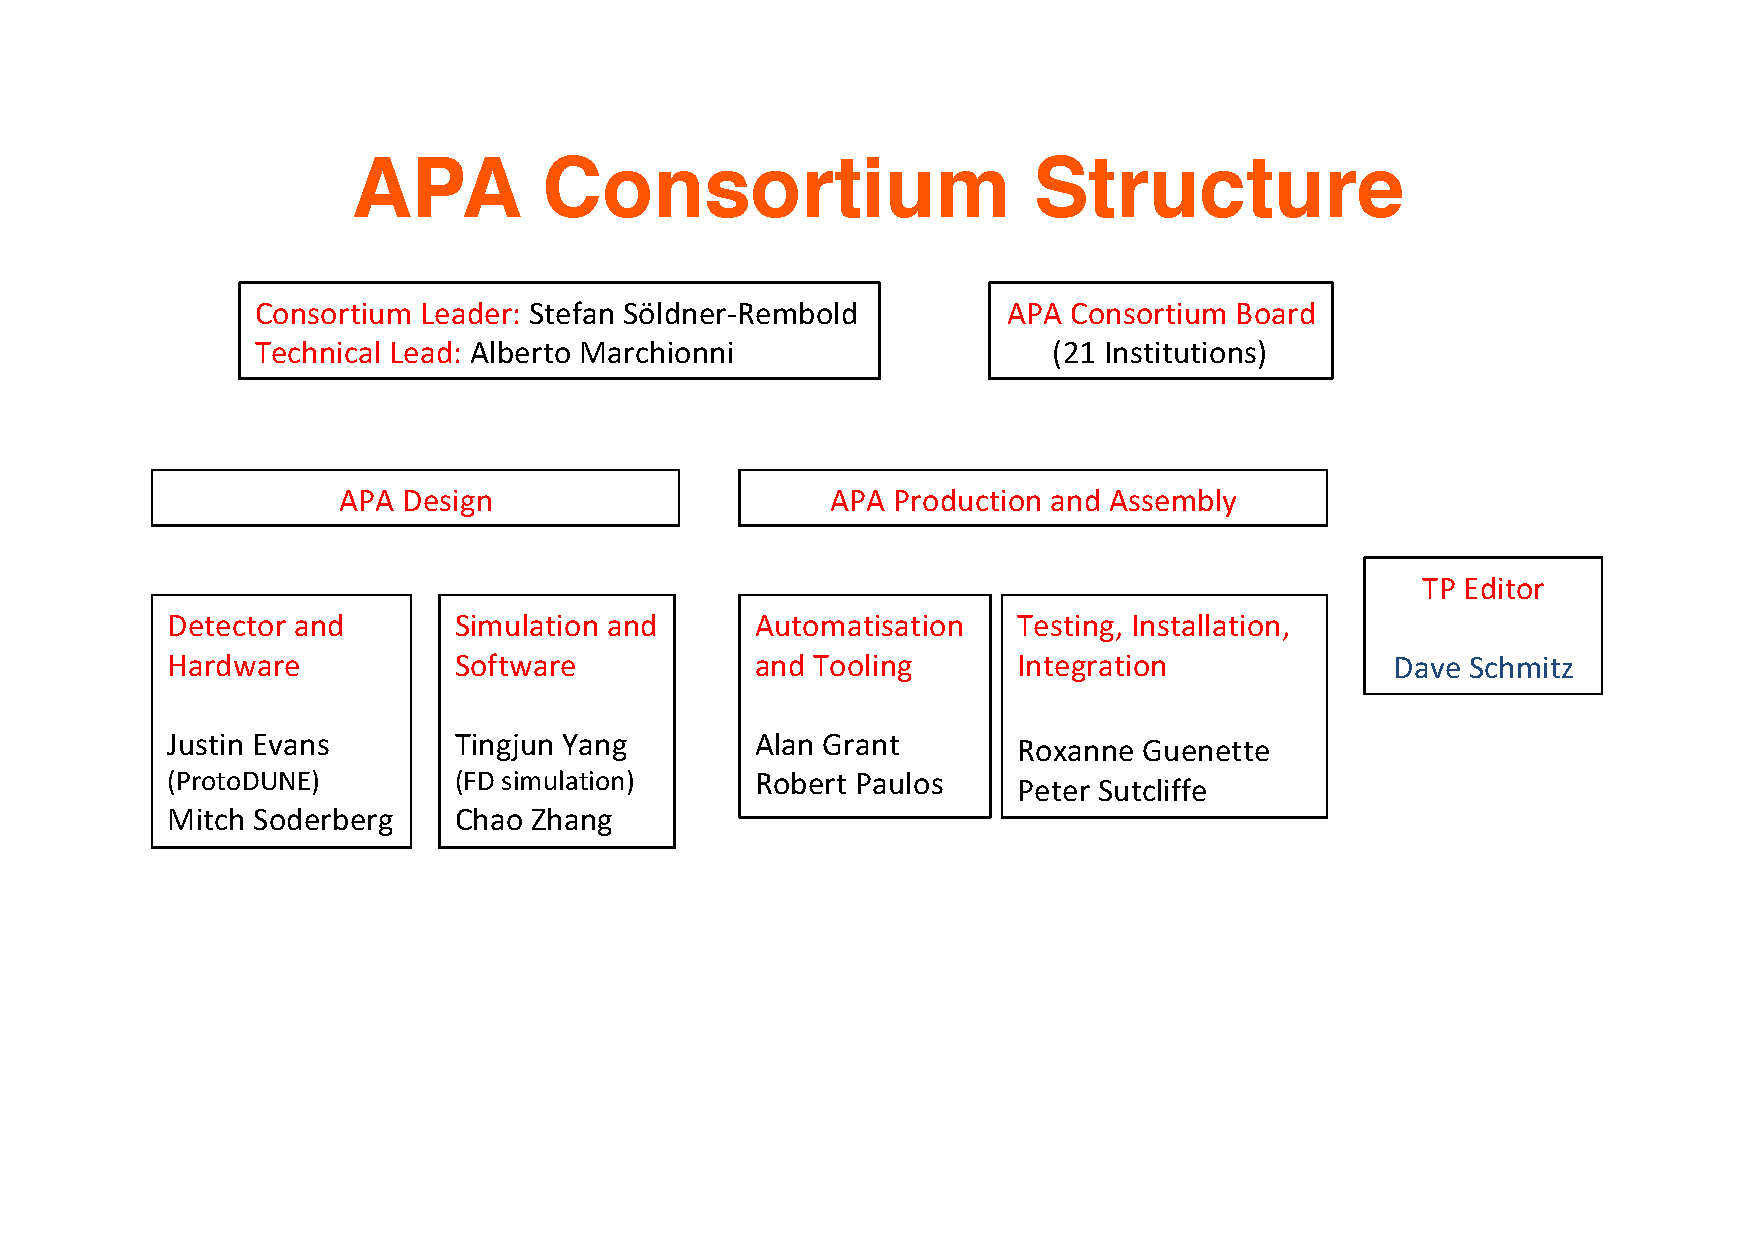
\includegraphics[width=0.9\textwidth,trim=0mm 60mm 0mm 15mm,clip]{Org_chart_no_frame.pdf}
\end{dunefigure}


%%%%%%%%%%%%%%%%%%%%%%%%%%%%%%%%%%%%%%
\subsection{Planning Assumptions}
\label{sec:fdsp-apa-org-assmp}
The planning assumptions are based on having 8-9 APA assembly lines, at different locations in the UK and the US. It will take of the order 50 shifts to construct a single APA. Assuming a multi-shift system, we will be able to construct the 150 APAs required for one 10 kt module within two years.


%%%%%%%%%%%%%%%%%%%%%%%%%%%%%%%%%%%%%%
\subsection{WBS and Responsibilities}
\label{sec:fdsp-apa-org-wbs}
\fixme{needs to be completed}

%%%%%%%%%%%%%%%%%%%%%%%%%%%%%%%%%%%%%%%
\subsection{High-level Milestones and Schedule}
\label{sec:fdsp-apa-org-cs}
\fixme{Our understanding is that there will be no Cost information in this document?}

\begin{dunetable}[Milestones]{ll}{tab:milestones}{Milestones}
Date &  Milestone   \\ \toprowrule
\multicolumn{2}{c}{Pre-TDR}\\
 December 2018 & Test 2-APA Assembly   \\
 January 2019 & Formal Review of complete Modifications to the Winder Design\\
 February 2019 & Formal review of protoDUNE APA performance \\
February 2019 & Complete assembly test of FD prototype APA\\
March 2019 & Decision on location of factories and required number of assembly lines \\
March 2019 & APA Cost Estimate for Far Detector 10 kt Module \\
March 2019 & APA schedule for Far Detector 10 kt Module \\
April 2019 & APA Section of Technical Design Report \\
\multicolumn{2}{c}{Post-TDR}\\
2020 & Preparation of APA factories \\
2021 -- 2023 & Construction of APAs \\
2022/3 & Installation of APAs in Far Detector 1\\
2024 & Commissioning of Far Detector 1 \\
\end{dunetable}